%%%%%%%%%%%%%%%%%%%%%%%%%%%%%%%%%%%%%%%%%
% Medium Length Professional CV
% LaTeX Template
% Version 2.0 (8/5/13)
%
% This template has been downloaded from:
% http://www.LaTeXTemplates.com
%
% Original author:
% Trey Hunner (http://www.treyhunner.com/)
%
% Important note:
% This template requires the resume.cls file to be in the same directory as the
% .tex file. The resume.cls file provides the resume style used for structuring the
% document.
%
%%%%%%%%%%%%%%%%%%%%%%%%%%%%%%%%%%%%%%%%%

%----------------------------------------------------------------------------------------
%	PACKAGES AND OTHER DOCUMENT CONFIGURATIONS
%----------------------------------------------------------------------------------------

\documentclass{resume} % Use the custom resume.cls style

\usepackage[left=0.75in,top=0.6in,right=0.75in,bottom=0.6in]{geometry} % Document margins
% \usepackage[utf8x]{inputenc} 
\usepackage{CJKutf8} 
\usepackage{pdfpages}
\usepackage{graphicx}
\name{Zhuowei Han} % Your name
\address{Pfaffenwaldring 44D, 70569, Stuttgart, Germany} % Your secondary addess (optional)
\address{+49/(0)176-61891464 or hanzhuowei1226@gmail.com} % Your phone number and email


\begin{document}
\begin{CJK*}{UTF8}{gbsn}
%----------------------------------------------------------------------------------------
%	OBJECTIVE SECTION
%----------------------------------------------------------------------------------------
 
\begin{rSection}{求职意向} 

算法工程师

\end{rSection}


%----------------------------------------------------------------------------------------
%	Summary 
%----------------------------------------------------------------------------------------
 
\begin{rSection}{职业技能}  
\begin{itemize}
\item 熟悉模式识别、机器学习算法和概率论、凸优化模型及其在语音识别和深度学习领域的应用
\item 扎实数字信号处理知识,有企业和学校项目实践经验
\end{itemize}
\end{rSection}

%----------------------------------------------------------------------------------------
%	WORK EXPERIENCE SECTION
%----------------------------------------------------------------------------------------

\begin{rSection}{研究经历}

\begin{rSubsection}{硕士论文,  题目:基于深度神经网络的语音情感识别 (英语)
}{2014/08 - 2015/02}{系统理论与信号处理学院,斯图加特大学}{}

\item 语音信号处理,提取MFCC特征作为语音情感低级特征
% \item Evaluated spectrum features of speech signals based on different database.
% \item Intergrated sparsity regularization to current the deep network to prevent overfitting.
\item 建立条件概率图模型(Conditional RBM)用以高级特征的非监督学习,建立多个基于深度神经网络的分类器模型并比较其性能
\item 优化模型参数及项目代码(Python)
% \item Fixed bugs in current Framework (Python).

\end{rSubsection}

%------------------------------------------------

\begin{rSubsection}{研究性论文, 题目:超声波传感器测距系统中的自适应门限参数优化 (德语)}{09/2013-03/2014}{罗伯特$\cdot$博世(德国)有限公司}{}
\item 超声波传感器的信号处理,根据参数优化目标设计并执行试验,分析试验数据并优化自适应门限参数和物体检测算法
\item 结合Excel-VBA与Matlab实现数据自动分析
\end{rSubsection}

%------------------------------------------------

\begin{rSubsection}{学生实验项目, 题目:基于统计学的汽车雷达信号处理 (英语)
}{09/2013-01/2014}{系统理论与信号处理学院,斯图加特大学}{}

\item 雷达信号处理,物体距离检测,基于卡尔曼滤波器的物体跟踪
\item 代码管理及维持项目进度,撰写提交研究报告

\end{rSubsection}

% \begin{rSubsection}{学生研究员}{04/2013-07/2013}{Student Employee}{Institute of High-Frequency Technology, University of Stuttgart}
% 
% \item 设计Matlab-GUI工具用于天线数据分析,通过Excel-VBA实现办公自动化
% % \item Studied the theory of frequency-domain Full Waveform Inversion. 
% 
% \end{rSubsection}
\end{rSection}


%----------------------------------------------------------------------------------------
%	EDUCATION SECTION
%----------------------------------------------------------------------------------------
\begin{rSection}{教育背景}
\begin{tabular}{l l}
 
{\sl 硕士,} & 电子信息工程\\
\end{tabular}

斯图加特大学,德国 \hfill 2012/10-2015/05 \\

\begin{tabular}{l l}
{\sl 本科,} & 电子信息工程\\
\end{tabular}

西安电子科技大学,西安 \hfill  2008/09-2012/07\\



\end{rSection}

%----------------------------------------------------------------------------------------
%	COMPUTER SKILLS SECTION
%----------------------------------------------------------------------------------------
\begin{rSection}{计算机技能}
\begin{tabular}{l l}
{\sl 编程语言:} &熟练掌握 Python, Matlab, VBA, 了解C++, Javascript, HTML+CSS\\
{\sl 工具:} &Git, Vim, Theano, \LaTeX{}, MS-Office
\end{tabular}

\end{rSection}

%-------------------------------Languages
%----------------------------------------------------------------------------------------
\begin{rSection}{语言技能}
中文(母语), 英语(熟练), 德语(熟练)
\end{rSection}

%----------------------------------------------------------------------------------------



%----------------------------------------------------------------------------------------
%	EXTRACURRICULAR ACTIVITIES SECTION
%----------------------------------------------------------------------------------------
% \begin{rSection}{EXTRACURRICULAR  ACTIVITIES}
% 
% Rohde\&Schwarz Case Study 2013, Participant. \hfill 05/2013 \\
% Intercultural Mentoring Program, University of Stuttgart, Mentee. \hfill 2012-2013 \\
% % 05/2014 \quad MOCHA marine MT deployment  Oregon Offshore, Volunteering\\	
% % 03/2014 \quad Seafloor Electromagnetic Methods Consortium, Presenting \\
% % 12/2013 \quad American Geophysical Union Annual Meeting, San Fransisco\\
% % 11/2013 \quad Nvidia GPU Workshop, San Diego Supercomputer Center\\
% % 08/2013 \quad Discover Big Data Workshop, SDSC 2013 Summer Institute\\
% % 06/2013 \quad MPI Workshop by  XSEDE, UC Los Angeles\\
% % 06/2013 \quad UCSD Triton 5K Running 
% 
% \end{rSection}

%----------------------------------------------------------------------------------------
%	HONORS AND  AWARDS
%----------------------------------------------------------------------------------------
% \begin{rSection}{HONORS AND  AWARDS}
% 
% 2012  \quad \quad RA Scholarship, UCSD/SDSU\\
% 2011  \quad \quad Erasmus Scholarship, EACEA\\
% 2011  \quad \quad Outstanding Student Scholarship, USTC\\
% 2010  \quad \quad National Aspiration Scholarship.\\
% %2010  \quad \quad Outstanding Student Scholarship, USTC\\
% 2009  \quad \quad Outstanding Student Scholarship, USTC\\
% 2008  \quad \quad Provincial Champion in Mathmatics, National College Entrance Exam.
% 
% \end{rSection}

\clearpage\end{CJK*}
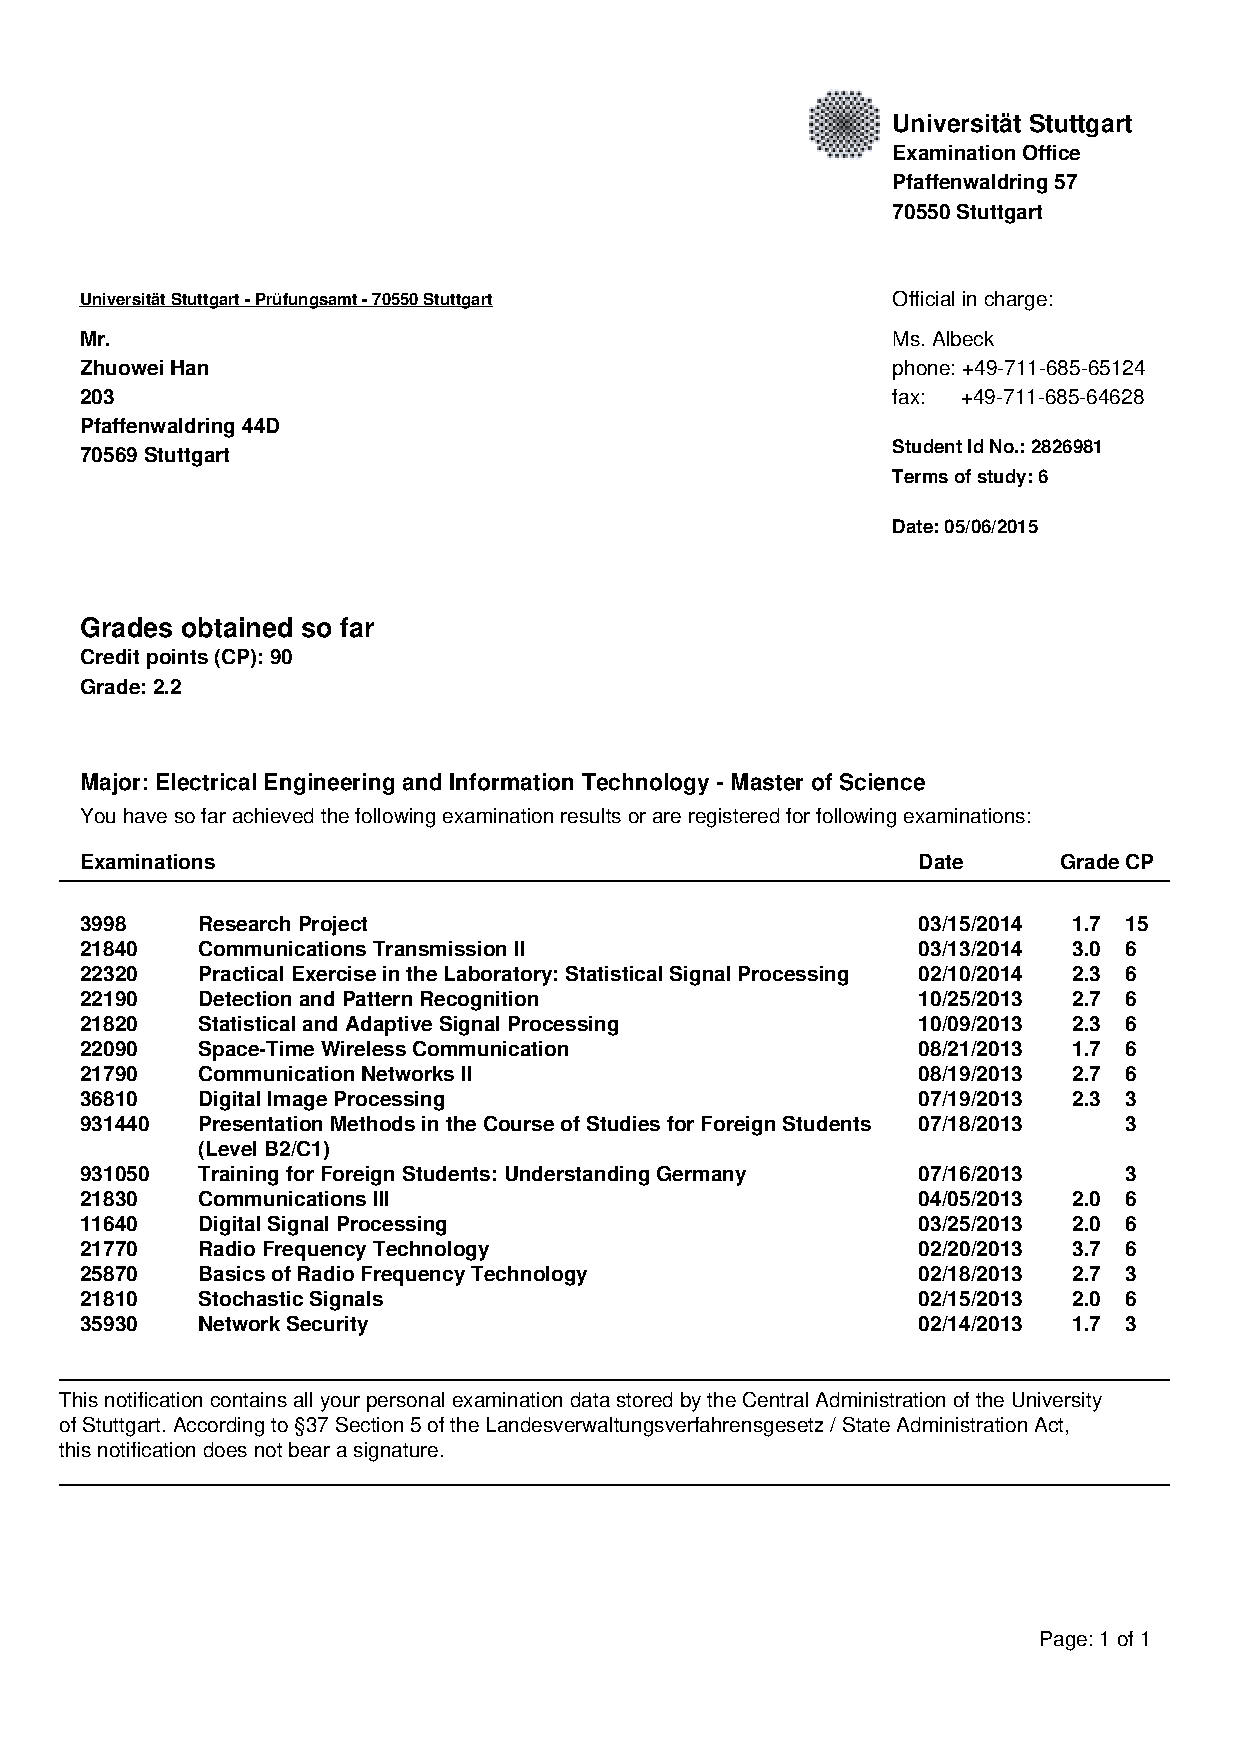
\includepdf[pages=-]{../Certificates/GradingMasterHan.pdf}
\Large Tranform from german grading to GPA\\
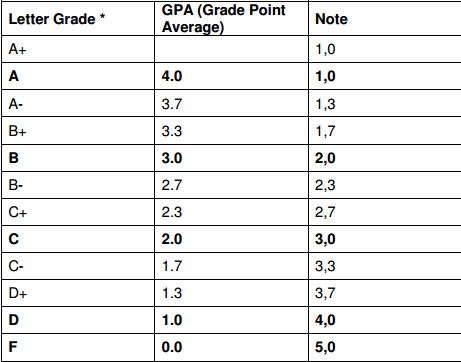
\includegraphics{../Certificates/GermanyGradingToUSA-GPA.png}
\end{document}
